\documentclass[11pt,a4paper]{report}
\usepackage[utf8]{inputenc}
\usepackage[T1]{fontenc}
\usepackage[english, italian, croatian]{babel}
\usepackage{amsmath, amsfonts, amssymb}
\usepackage{graphicx}
\usepackage{fancyhdr}
\usepackage{color}
\usepackage {tikz}
\usepackage{pgfplots}
\usetikzlibrary {positioning}
\usepackage{tocloft}
\usepackage[hidelinks]{hyperref}
\usepackage[section]{placeins}
\usepackage[final]{pdfpages}
\bibliographystyle{ieeetr}%ieeetr, abbrv
\pgfplotsset{compat=1.15}
\usepackage{listings}
\usepackage{appendix}
\usepackage{lipsum}
%\usepackage{chngcntr}	%Continuous footnote numbering
%\counterwithout{footnote}{chapter} %Continuous footnote numbering
\tolerance=1
\emergencystretch=\maxdimen %poravnavanje
\hyphenpenalty=10000 % no hyphenation
\hbadness=10000	

\renewcommand{\cftsecleader}{\cftdotfill{\cftdotsep}}
\addto{\captionscroatian}{\renewcommand{\bibname}{Literatura}}
%\setcounter{chapter}{-1} % zero-based numbering
\pagenumbering{Roman}

\newcommand{\kolegij}{Završni rad}
\newcommand{\naslovRada}{Izrada snimača podataka, obrada i vizualizacija prikupljenih podataka bazirana na principima slobodnog i otvorenog koda \\ {\large Završni rad}} 
\newcommand{\mailFriendlynaslovRada}{BachelorThesis - FOSS Datalogger}

\author{
Kristijan Cetina \\{\small JMBAG: 2424011721} \\ {\href{mailto:kristijan.cetina@gmail.com?subject=\mailFriendlynaslovRada}{{\footnotesize kcetina@iv.hr}}}} 
\title{\naslovRada}
\date{Pula, \today}

\begin{document}
\pgfplotsset{width=\textwidth,compat=newest}

\begin{titlepage}
\clearpage
\begin{center}
\begin{Large}
ISTARSKO VELEUČILIŠTE\\
UNIVERSIT\`{A} ISTRIANA DI SCIENZE APPLICATE\\
Stručni studij politehnike\end{Large}
\end{center}
\vspace{3cm}
{\let\newpage\relax\maketitle}
\thispagestyle{empty}

\begin{abstract}
Prikupljanje, obrada i vizualizacija podataka nalazi se na svakom koraku našega života.
U ovom radu prikazan je postupak izrade snimača podataka koristeči Arduino platformu te obrada podataka koristeći iskljućivo alate otvorenog i slobodnog koda.
Hardwareska platforma trenutno koristi GPS prijemnik i temperaturni senzor te se u budućnosti planira povećanje broja senzora.
Podatci koji se skupljaju na uređaju spremaju se lokalno na memorijsku karticu ne bi li se kasnije analizirali na računalu pri čemu se koristi programski jezik Python unutar Jupyter notebook okruženja uz pomoć Pandas, NumPy i Matplotlib biblioteka.
Izrađeni alat za analizu radi na svim popularnim operacijskim sustavima danas u upotrebi.

U duhu otvorenog koda i dobre prakse znanstvene zajednice ovaj rad je napisan koristeći \LaTeX{} sustav te je kompletan rad \textit{hostan} na GitHub-u i slobodano dostupan svim zainteresiranim stranama koji žele nastaviti rad na ovoj temi.

\paragraph{Ključne riječi} \textit{Arduino, Python, Matplotlib, \textit{open-source}, obrada podataka}
\vspace{3cm}

\begin{tabbing}
\hspace{60pt}\=\kill
 Kolegij: \> Elektronika\\
 Mentorica: \> Sanja Grbac Babić, mag. računarstva, v.predavač
\end{tabbing} 
\end{abstract}

\begin{otherlanguage}{italian} 
\begin{abstract}
La raccolta, l’elaborazione e la visualizzazione dei dati è presente in ogni aspetto della nostra
vita.
In questa tesi è documentata la creazione di uno strumento per la raccolta dati creato su
piattaforma Arduino, e l’elaborazione dei dati raccolti usando esclusivamente strumenti \textit{Open Source}.
La piattaforma hardware attuale usa un ricevitore GPS ed un sensore di temperatura mentre per future evoluzioni è in programma l’incremento del numero di sensori. 
I dati raccolti dallo strumento vengono immagazzinati sulla scheda di memoria per poi essere analizzati sul computer.
Per l’analisi dei dati viene usato il linguaggio di programmazione Python sull' ambiente di programmazione Jupyter notebook, con l’ausilio di biblioteche Pandas, NumPy e Matplotlib.
Lo strumento qui descritto è compatibile con tutti i sistemi operativi piu popolari oggi in uso.

Nello spirito della filosofia Open Source e della cultura scientifica questa tesi e stata scritta usando il sistema \LaTeX{} ed è disponibile liberamente su GitHub per tutti coloro che fossero interessati a continuare il lavoro fatto su questo tema.

\paragraph{Parole chiave:} \textit{Arduino, Python, Matplotlib, \textit{open-source}, analisi dati}
\end{abstract}
\end{otherlanguage}

\begin{otherlanguage}{english} 
\begin{abstract}
Data acquisition, processing, and visualization are at every step of our lives.
This paper describes how to record data using an Arduino and analyze them using free and open-source (FOSS) tools exclusively.
The hardware platform is currently using a GPS receiver and a temperature sensor with the planned increase in the number of sensors in the future.
The data collected on the devices is stored locally to a memory card and subsequently analyzed on a computer.
The Python programming language within the Jupyter notebook environment was used for analysis with the help of the Pandas, NumPy and Matplotlib libraries.
The created analysis tool works on all today popular operating systems.

In the spirit of the open-source and good practice of the scientific community, this paper was written using the \LaTeX{} system and a complete project is hosted on GitHub freely available to all interested parties who wish to work on these topic.

\paragraph{Keywords:} \textit{Arduino, Python, Matplotlib, \textit{open-source}, data analysis}
\end{abstract}
\end{otherlanguage}

\end{titlepage}

\vspace*{\fill}
\begin{flushright}
\textit{Mojoj mami Vlasti}
\end{flushright}
\vspace*{\fill}
\chapter*{Zahvala}
Zahvaljujem s svojoj mentorici Sanji Grbac Babić, mag. računalstva, viši predavač na izdvojenom vremenu i podršci kako na izradi ovog rada tako i tijekom cijelog studiranja na Politehnici.
Svojm smirenim pristupom uvelike je olakšala proces učenja i rada bilo da se radilo o stručnim tehničkim pitanjima ili ostalim izazovima koji se studenti susreću.

Zahvaljujem se i svojim timskim kolegama Stjepanu Grginu i Igoru \mbox{Mrkiću} s kojima sam od samog početka sudjelovao na svim timskim zadacima i njihovoj pomoći pri individualnom radu. 
Team \textit{One} rocks.

Zahvaljujem se i svim ostalim profesorima i djelatnicima Politehnike koja je tokom studija narasla i preimenovana u Istarsko Veleučilište - Universit\`{a} Istriana Di scienze applicate na nesebičnoj potpori kada je god to bilo potrebno.
Vi činite ovu ustanovu ono što ona je.

Naposljetku veliko hvala mojoj obitelji na svoj potpori i razumjevanju tokom mojeg ponovnog studiranja.
Draga mama, iako više nisi s nama znam da biš bila sretna.

\vspace*{2cm}

\begin{quotation}
"A good scientist is a person with original ideas. A good engineer is a person who makes a design that works with as few original ideas as possible. There are no prima donnas in engineering" - Freeman Dyson
\end{quotation}
\section*{Izjava o samostalnosti izrade završnog rada}
Izjavljujem da sam završni rad na temu "GPS datalogger" samostalno izradio uz pomoć mentorice Sanje Grbac Babić mag. računarstva, koristeći navedenu stručnu literaturu i znanje stečeno tijekom studiranja. Završni rad je pisan u duhu hrvatskog jezika.
\vspace{\fill}
\begin{flushright}
Student: Kristijan Cetina\\
\vspace{15mm}
--------------------------------------------------------------
\end{flushright}

\tableofcontents
%\listoftables	%ako ih ima puno prebaci na kraj dokumenta
\listoffigures	%ako ih ima puno prebaci na kraj dokumenta
\newpage

\pagenumbering{arabic}
\chapter{Uvod i opis zadatka}\label{OpisIOgranicenja}

\section{Opis i definicija problema}

\section{Cilj i svrha rada}
Cilj ovog rada je bio izraditi jednostavan snimač podataka (\textit{datalogger}) koji će spremati GPS podatke zajedno s podacima prikupljenim sa instaliranih senzora za kasniju analizu.
Izrađeni uređaj je namjenjen kao snimač podataka u kompleksnijem sklopu koji je koji se može koristiti kda god postoji potreba za loggiranje podataka.
Uređaj je namjenjen da zadovolji široki spektar potreba koje se mogu javiti bilo u industriji npr. prilikom praćenja pošiljki ili pak prilikom skupljanja podataka u istraživačke svrhe kako bi se razumio širi problem.

Sklop je baziran na Arduino platformi koja omogućava lak razvoj prototipova uz široku dostupnost gotovih dodatnih modula (\textit{shields}) koji se jednostavno spajaju na bazno mikroračunalo.

Prikpljeni podaci se spremaju na SD karticu na uređaju u datoteku za kasniju obradu i analazu.
Prikupljeni podaci se uz pomoć programskog jezika Python i dodatnih modula za statističku i numeričku analizu kao što su Pandas i Matplotlib obrađuju kroz sučelje interaktivne bilježnice Jupyter Notebook.
Pristup obrade putem interaktivne bilježnice uz korištenje raznih tipova čelija kao što su \textit{Code Cells, Markdown Cells i Raw Cells} omogućava lakšu vizualizaciju i pregled samog rada koji je pogodan za kasnije dijeljenje svim zainteresiranim stranama koji žele pregledati ili nastaviti rad na analizi.

\section{Hipoteza rada}

\section{Metode rada}

\section{Struktura rada}
Kompletan Git repozitorij ovog rada javno je dostupan na \url{https://github.com/KristijanCetina/BachelorThesis}
\chapter{Opis korištenih tehnologija}\label{technologyStack}
\section{Slobodan i otvoreni kod}
Izraz otvoreni kod (\textit{open source}) odnosi se na nešto što ljudi mogu slobodno mijenjati i dijeliti jer je dizajn javno dostupan\cite{WhatIsOpenSource}.
Izraz je nastao u kontekstu razvoja računalnog softwarea dok se danas odnosi na pristup radu bio on software, hardware ili bilo kakav drugi tip projekta.
Spomenimo kako postoje razne licence pod kojima se objavljuju open soure radovi, a u praksi se razlikuju u načinu na koji izmjenjeni i izvorni rad mora biti distribuiran svim ostalim zainteresiranim stranama.

Razlozi i prednosti primjene open source pristupa projektima su višestruke, a neke od njih su:
\begin{itemize}
\item Kontorla proizvoda
\item Učenje i trening
\item Sigurnost
\item Stabilnost
\end{itemize}

\paragraph{Kontrola proizvoda:}
Kada je izvorni kod i ostala dokumentacija nekog proizvoda otvorena onda se može pogledati kako točno radi taj proizvod i na koji način je izgrađen.
Na taj način svaki korinik može imati kontrolu nad onime što koristi jer ne postoji koncept crne kutije (\textit{BlackBox concept}) te omogućava korisniku da uz dostupan kod i sheme popravi ili unaprijedi proizvod.
Zapitajmo se koliko puta smo se osobno susreli sa situacijom kada zbog kvara nekog uređaja smo bili primorani posjetiti i platiti ovlaštenog servisera koji ima specijalni alat za diagnostiku i popravke?

\paragraph{Učenje i trening:}
Uvidom u otvorenu dokumentaciju možemo vidjeti kako je neki stručnjak rješio određeni problem te to rješenje u potpunosti ili modificirano može se primjeniti na vlastiti problem.
Otvorena dokumentacija omogućava proučavanje rješenja određenih problema i na taj način se skračuje vrijeme i pojeftinjuje razvoj novih proizvoda koji imaju slične zahtjeve.
Znanstvenici objavljuju svoja otkrića kako bi ih drugi iza njih mogli koristiti.
Inženjeri u svakodnevnom radu ne izvode i dokazuju npr. Ohmov ili Newtonove zakone već ih samo primjenjuju.

\paragraph{Sigurnost:}
Proučavanje objavljene dokumentacije nekog projekta drugi stručnjaci iz područja mogu uvidjeti neke propuste koje autori zbog kompleksnosti proizvoda ili drugih razloga nisu primjetili te dojaviti autorima grešku kao bi se ista mogla ispraviti. 
Neke greške se mogu pojaviti samo u iznimno malom broju slučaja ili kada se poslože veliki broj faktora te nije realno očekivati da se prilikom testiranja proizvoda simulira svaki mogući scenarij korištenja.
Zainteresirane strane mogu dodatno testirati proizvod u specifičnim uvjetima i na taj način otkriti inače skrivenu grešku u proizvodu te nakon otklanjanja greške sam proizvod postaje sigurniji.

\paragraph{Stabilnost:}
Mnogi proizvodi se koriste za vrlo bitne aspekte rada nekog većeg sustava te njihova zamjena iziskuje velike promjene i investicije, a ponekada nije niti moguća.
Korištenjem proizvoda otvorenog koda i dokumentacije omogućava se korištenje nastavak podrške i korištenja tog proizvoda i nakon eventualnog nestanka kompanije koja je napravila proizvoda te isti više nije dobaljiv od proizvođača. 
Ako se koriste open source proizvodi moguće je samostalno rekreirati proizvod ukoliko se ukaže takva potreba.


\section{Arduino platforma}
Arduino je elektronička platforma otvorenog koda\footnote{\url{https://www.arduino.cc/en/Guide/Introduction}} bazirana na hardwareu i softwareu koji je lako za koristiti.
Arduino platforma obuhvaća mikrokontrolerske pločice bazirane na AVR arhitekturi s integriranim digitalnim, alalognim ulazima i izlazima kao i PWM\footnote{Pulse Width Modulation - Pulsno širinska modulacija} izlazima.
Platforma omogućava lagano spajanje dodatnih vanjskih uređaja kao što su razni senzori, releji, servo i motori putem dodatnog upravljačkog modula i ostale elektroničke i elektromehaničke komponente.
Sheme svih mikrokontrolera objavljene pod Creative Commons\footnote{\url{https://creativecommons.org/}} licencom i javno dostupne svim zainteresiranim stranama.

Adruino pločice su relativno povoljne u usporedbi s ostalim platformama i kao takve omogućavaju pristupačnije učenje svim zainteresiranima.
Potrebno je ponekad malo spretnosti s lemilicom dok se često mogu slagati moduli na prototipnoj pločici bez lemljenja sa izradom spojeva putem spojnih žica.

Jednostavno korisničko sučelje (IDE\footnote{Integrated development environment - Integrirano razvojno okruženje}) za izradu korisničkih programa (\textit{sketch}) je jednostavno za korištenje za početnike dok istovremeno omogućava izradu vrlo kompleksnih programa iskusnim korisnicima. 
IDE je kompatibilan s većinom danas raspostranjenih operacijskih sustava (GNU/Linux, MacOS i Windows).
Programski jezik za izradu programa je baziran na C/C++ te omogućava daljnje proširivanje kroz C++ biblioteke ili koristiti AVR-C programski jezik.

\section{Jupyter Notebook}
U ovom radu za obradu i prikazivanje podataka korišten je programski jezik Python\footnote{\url{https://www.python.org/}} uz dodatke NumPy\footnote{\url{https://numpy.org/}}, Pandas\footnote{\url{https://pandas.pydata.org/}} i Matplotlib\footnote{\url{https://matplotlib.org/}}.
NumPy i Pandas omogućavaju lakšu manipulaciju podacima dok Matplotlib omogućava izradu kvaitetnih grafova s velikom mogučnošću prilagodbe raznim željama i potrebama.
Sve zajedno je implementirano kroz sustav \emph{interaktivne bilježnice} Jupyter\footnote{\url{https://jupyter.org/}} koja omogućava brzu i jednostavnu obradu podataka kao i njeno dijeljenje sa svim zainteresiranim stranama.
Jupyter notebook je web aplikacija otvorenog koda koja se može izvršavati na lokalnom računalu ili koristeći resurse računalstva u oblaku.
Podržava razne programske jezike poput Julia, Ruby, R, C++ i mnoge druge te u ovom radu korišten Python.
Jupyter notebook omogućava kreiranje i djeljenje dokumenata koji sadržavaju izvršivi programski kod, jednadžbe, grafove i vizualizacije te popratni tekst u jednoj cijelini koju trenutno drugim načinima nije moguće ili je vrlo nepregledno za postići.
Područja primjene su najčešće obrada i transformacija podataka, numeričke analize, statistički modeli, vizualizacija podataka, strojno učenje i još mnogo toga.

Alati tipa Excel gdje korištene formule su skrivene iza podataka u ćelijama te se greške lako podkradu i još lakše ostanu nezamječene. 
Istraživanja su pokazala značaju količinu grešaka u Excel proračunskim tablicama koje su u dnevnoj upotrebi diljem organizacija, od kojih neke su imale i značajne negativne financijke implikacije\cite{panko1998we}. 
Iako je istraživenje starijeg datuma jedan od glavnih razloga grešaka (skrivene formule) je i dalje prisutan te je realno za očekivati kako se greške i dalje događaju, a sa sve većom upotrebom proračunskih tablica za očekivati je kako broj istih s greškama raste.

Primjenom interaktivnih alata poput Jupyter notebooka koji imaju vidljivo prikazane formule koje koriste za proračun i kod kod za manipulaciju podataka lakše se mogu uočiti greške unutar istih te se mogu ispraviti.
Primjenom metodologije testiranja koja je poznata u industriji raznova softwarea greške se mogu dodatno smanjiti.
Jedan od poznatijih projekata analize velike količine podataka je zasigurno detekcija gravitacijskih  valova nastalih spajanjem dvaju crnih rupa koristeći LIGO teleskop (\textit{Laser Interferometer Gravitational-Wave Observatory})\footnote{\url{https://www.gw-openscience.org/tutorials/}}

\section{NumPy}
NumPy je fundamentalni paket za numeričku analizu koristeći Python.
Izmežu ostalih funkcija sadrži
\begin{itemize}
\item snažan alat za rad s N-dimenzionalnim poljima
\item alat za intergraciju C/C++ i Fortran programskog koda
\item korisne alate za algebarske operacije, Fourierovu analizu i ostale numeričke mogućnosti
\end{itemize}

Osim što značajno olakšava numerički i statističku analizu skupa podataka NumPy zbog svoje strukture i reprezentacije polja podataka omogućava značajno poboljšanje performansi obrade podataka.
Kako bi demonstrirali razliku u performansama između čistog Pythona i NumPy biblioteke možemo napraviti jednostavan eksperiment koji se sastoji od sumiranja elemenata u polju veličine $10^6$ elemenata i mjeriti vrijeme potrebno za izvršavanje tog zadatka.

\begin{figure}[!h]\begin{center}
\includegraphics[width=1\textwidth]{{"../resources/npSpeedTest"}.png}
\caption{Usporedba performanski Pythona i NumPy biblioteke}\label{data:npSpeedTest}
\end{center}\end{figure}
Na slici \ref{data:npSpeedTest} prikazana je razlika u brzini izvršavaja operacija sumiranja zadanog polja elemenata.
Vrijeme potrebno za sumiranje elemenata koristeći samo Python iznosi $26.8 ms \pm 750 \mu s$ dok koristeći NumPy vrijeme za isti zadatak iznosi samo $403\mu s \pm 2.46\mu s$\footnote{Rezultati mogu varirati u zavisnosti o korišenom računalu}.
Vidljiva je značajna razlika u potrebnom vremenu za izvršavanje zadatka, a iskusva industrije\cite{van2011numpy} pokazuju još veću razliku kod kompleksnijih zadataka.

\section{Git}
Git\footnote{\href{https://git-scm.com/}{https://git-scm.com/}} je distribuirani sustav za verzioniranje koda i ostalog rada kojeg želimo djeliti sa suradnicima.
Git sa svojim jednostavnim i brzim granama omogućava lakši razvoj proizvoda kao i ispitivanje mogućnosti i funkcija.
Kada se želi ispitati neka funkcionalnost bez da se ugrozi ono što do sada radi kako trebe nema potrebe kopirati cijeli projekt u novi folder i onda u njemu testirati već se jednostavno kreira nova grana u kojoj se radi razvoj i kada smo sigurni da sve radi kako želimo onda se ta grana ujedini s glavnom granom projekta koja prihvati dodatne funkcionalnosti koje su razvijene za proizvod.
Kako je Git lagan za resurse onda se može kreirati vrlo veliki broj grana za razne potrebe bez značajnog utjecaja na performanse razvojnog računala ili potrošnje spremišnog prostora.

S obzirom na distibuiranu narav Gita svaki suradnik koji radi na projektu ima svoju kopiju na kojoj radi te nije vezan za neki server i stalnu komunikaciju s ostatkom tima već je ista potrebna samo kada se povlače i šalju učinjene promjene.

Git je nastao 2005 godine za potrebe razvoja Linux jezgre i od tada je poprimio mnoge simpatije unutar inženjerske zajednice koja ga koristi kako bi zajednički razvija projekte.

Kako bi se olakšalo djeljenje i suradnja na projektima 2008. godine je pokrenut GitHub - centralno mjesto za usluge poslužitelja\footnote{\href{https://github.com/features}{https://github.com/features}} (\textit{hosting}) putem kojeg je moguće pratiti životni ciklus i povijet projekta.
Svatko može pronaći projekt koji ga zanima te ukoliko ima dovoljno vremena i znanja može i pridonjeti njegovom razvoju.
Brojne kompanije koriste GitHub kao bi podjelile svoje projekte. Podatak od travnja 2019. godine kaže kako više od 2.1 miljuna kompanija i organizacija koristi GitHub.
Jedna od njih je i Adafruit - kompanija koja proizvodi elektroničke dodatke za Arduino i druge platforme i fokusirana je na edukacija mladih (i onih koji se tako osjećaju), a njihov GitHub sadrži više od 1100 repozitorija\footnote{\href{https://github.com/adafruit}{https://github.com/adafruit/}}.
Upravo je njihov GPS Logger Shield korišten u ovom projektu, a dostupnos dokumentacije i dostupna podrška je jedan od glavnih razloga zašto je odlučeno koristiti upravo taj proizvod.

\chapter{Prikupljanje podataka - hardware}
\begin{figure}[h]
\begin{center}
\includegraphics[width=1\textwidth]{{"../resources/HardwareSetup"}.jpg}
\caption{Izgled korištenog hardwareskog sklopa}\label{pic:HardwareSetup}
\end{center}
\end{figure}

\section{GPS logging shield}

\begin{figure}
\begin{center}
\includegraphics[width=0.7\textwidth]{{"../tempSensor/TMP36_schematic"}.jpg}
\caption{Shema spoja TMP36 senzora}\label{shema:TMP36}
\end{center}
\end{figure}

\begin{figure}
\includegraphics[angle=90,width=1.1\textwidth]{{"../Adafruit-GPS-Logger-Shield-PCB/Adafruit GPS Logger Shield"}.pdf}
\caption{Shema Adafruit GPS Logger Shield}\label{shema:AdafruitLoggerShield}
\end{figure}

Na shemi \ref{shema:AdafruitLoggerShield} nalazi se shema gotovog elektroničkog sklopa kako dolazi iz tvornice\footnote{Kompletna dokumentacija dostupna je na \url{https://learn.adafruit.com/adafruit-ultimate-gps-logger-shield?view=all}}\footnote{GitHub repozitorij korištene verzije dostupan na \url{https://github.com/adafruit/Adafruit-GPS-Logger-Shield-PCB}}.
Na samoj tiskanoj pločici postoji tkz. prototipno područje za dodavanje vanjskih elemanata čiji je raster 2.54 mm koji odgovara standardu \textit{true-hole} elemenata.
Na to područje je dodan temperaturni senzor TMP36\footnote{Datasheet dostupan na \url{https://github.com/KristijanCetina/BachelorThesis/blob/master/resources/TMP35_36_37.pdf}}\label{ftn:TMP36Datasheet} zajedno s dodatnim pasivnim elementima koji služe kao filter smetnji koje se javljaju u radu zbog okoline.
Shema spoja je prikazana na slici \ref{shema:TMP36}.

\section{Prikupljanje podataka o temperaturi}\label{sec:TempData}
Kako svaki elektronički sklop ima definirani raspon radne temperature bitno je znati u kojim uvjetima isti se nalazi.
Ukoliko je temperatura previsoka može se uključiti aktivno hlađenje ili ako se unaprijed zna da će se sklop nalaziti pod povišenom radnom temperaturom onda se može konstrurati adekvatan sustav hlađenja.
Isto vrijedi za prenisku temperaturu.
Prema ranije spomenutoj shemi \ref{shema:TMP36} dodatn je temperaturni senzor koji mjeri radnu temperaturu okoline uređaja.
Pri testiranju ova vrsta senzora se pokazala veoma pouzdana, uz minimalno samozagrijavanje koje bi utjecalo na točnost mjerene veličine ali je isto tako pokazala vrlo brze promjene izlazne vrijednosti koja može biti do vanjskih smetnji.
Kako bi se otklonio taj problem primjenjena su dva rješenja.
Prvi je hardwareski fiter - kondenzatori koji je prikazan na shemi \ref{shema:TMP36}, a drugi je softwareski fiter.
Tvornički podaci o izlaznom naponu šuma mogu se pronaći u datasheetu uređaja, slika 20.
Na slici \ref{data:RawWithOutCaps} prikazane su izlazne vrijednosti senzora bez ikakvog filtriranja i obrade.
frekvencija uzorkovanja je 10Hz (10 očitanja u sekundi)
Svakako nije realno za očekivati da se temperatura mjenja sukladno očitanim vrijednostima.

\subsection{Softwareski filter}
Softwareski filter radi na principu da očitava 10 vrijedosti sa senzora te ih sprema u polje.
Potom ih sortira po veličini i uzima medijan\footnote{Medijan (mediana, centralna vrijednost) je pojam iz statistike koji određuje sredinu distribucije. Pola vrijednosti skupa (distribucije) nalazi se iznad mediane, a pola ispod} vrijednost kao točnu temperaturu.
Na taj način se postiže da se eliminiraju sve vrlo visoke i vrlo niske vrijednosti koje se mogu pojaviti zbog šuma u signalu.
Vrijenosti se čitaju svakih 100 ms te uz račuanje na bazi 10 vrijednosti daje frekvenciju od 1 očitanja u sekundi koja odgovara i frekvenciji uzorkovanja podataka sa GPS senzora.
Prilikom testiranja utvrđeno je da veći broj uzoraka ne doprinosti kvaliteti izmjerenih vrijednosti, a pro manjem broju uzoraka može se potkrasti poneka nerealna vrijenosti.
Kako je očekivano vrijeme promjene temperature značajno duže od 1 sekune onda su prihvaćene navedene vrijednosti i metoda filtriranja.
Na slici \ref{data:FilteredWithOutCaps} prikazane su izlazne vrijendosti senzora nakon primjene opisanog softwareskog filtera.
Primjeti se značajno manje skokova od nečega što se može smatrati stvarna vrijendost. 

\begin{figure}[!h]
\begin{minipage}{0.49\linewidth}
\includegraphics[width=\linewidth]{{"../tempSensor/RawWithOutCaps"}.jpg}
\caption{Vrijednosti senzora bez \mbox{filtriranja}}\label{data:RawWithOutCaps}
\end{minipage}
\hfill
\begin{minipage}{0.49\linewidth}
\includegraphics[width=\linewidth]{{"../tempSensor/FilteredWithOutCaps"}.jpg}
\caption{Vrijednosti senzora sa \mbox{softwareskim} filtriranja}\label{data:FilteredWithOutCaps}
\end{minipage}
\end{figure}

\subsection{Hardwareski filter}
Filter je jednostavna mreža keramičkih kondenzatora vrijednosti $10 pF$ koji su spojeni što bliže senzoru između izvoda za napajanje i izlaza senzora prema točki nultog potencijala (\textit{GND, masa}) kako bi apsorbirali eventualne smetnje.
Iako je softwareski fiter u nekim situacijama dovoljno dobar ovo jednostavno i jeftino rješenje daje dodatan sloj filtriranja koji za posljedicu ima vrlo glatko očitanje temperature bez skokova u vrijednostima.

Primjenom kombinacije softwareskog i hardwareskog filtriranja postignuta je vrlo zadovoljavajuća karakteristika dobivenih stabilnih vrijednosti bez nerealnih skokova i s vrlo glotkom tranzicijom kod grijanja ili hlađenja sklopa. Dobivene vrijednosti su prikazane na slici \ref{data:FilteredWithCaps}.
\begin{figure}[!h]\begin{center}
\includegraphics[width=0.8\textwidth]{{"../tempSensor/FilteredWithCaps"}.jpg}
\caption{Vrijednosti senzora primjenom kombinacije Sw i Hw filtera}\label{data:FilteredWithCaps}
\end{center}\end{figure}

\section{Prikupljanje GPS podataka}
GPS\footnote{Global Positioning System - Sustav globalnog pozicioniranja} je javni sustav u vlasništvu vlade SAD-a\footnote{\url{https://www.gps.gov}} za globoalno pozicioniranje baziran na satelitima s atomskim satovima koji odašilju vrlo točno i precizno trenutno vrijeme te su sinkkronizirani s zemaljskim satovima. 
Bilo kakva odstupanja se korigiraju na dnevnoj bazi.
Prijemnik prima signal sa satelita te izračunava točnu poziciju baziranu na poznatoj poziciji satelita i razlikama u primljenim vremenima od svakog satelita.
Minimalno su potrebna 3 satelita za dobiti koordinate i 4 satelita za dobiti poziciju o nadmorskoj visini prijemnika.

U ovom radu korišten je GPS chip MTK3339\footnote{\url{https://cdn-shop.adafruit.com/datasheets/GlobalTop-FGPMMOPA6C-Datasheet-V0A-Preliminary.pdf}} integriran na prije spomenuti Adafruit Ultimate GPS Logger Shield.


Kao koristan izlaz prijemnik daje NMEA\footnote{\url{https://www.nmea.org/content/STANDARDS/NMEA_0183_Standard}} rečenicu. 
Ovisno o potrebnim podacima mogu se koristiti razne rečenice, a u ovoj primjeni je korištena \$GPRMC\footnote{\url{http://aprs.gids.nl/nmea/}} koja daje minimalne potrebne podatke, a među kojima su vrijeme (UTC) i datum, pozicija i brzina.
Primjer \$GPRMC rečenice je \begin{verbatim}
$GPRMC,053005.000,A,4457.8784,N,01356.1351,E,36.41,124.90,310719,,,A*58
\end{verbatim}
pri čemu je:
\begin{tabbing}
\hspace{80pt}\=\kill
 \$GPRMC \> Oznaka rečenice \\ 
 053005.000 \> UTC vrijeme (7:30:05 lokalno)\\ 
 A \> Oznaka valjanosti, A = OK, V = warning \\ 
 4457.8784,N \> Zemljopisna širina \\ 
 01356.1351,E \> Zemljopins dužina \\ 
 36.41 \> Brzina u čvorovima ($\approx 67 km/h$)\\ 
 124.90 \> Smjer kretanja \\
 310719 \> Datum (31. srpnja 2019.)\\
 A*58 \> Checksum (kontrolni broj)
\end{tabbing} 
Prilikom provjere primljenih podataka obavezno se provjerava
\begin{itemize}
\item da li primljni checksum odgovara izračunanom za datu rečenicu kako bi se izbjegle pogreške u komunikaciji,
\item da li je oznaka valjanosti \textit{A} što znači da uređaj ima prijem s dovoljnog broj satelita da se može vjerovati primljenim podacima.
\end{itemize}
Provjeru valjanosti i checksuma odrađuje bibloteka koja je dostupna za Arduino platformu zajedno s ostalom dokumentacijom uređaja te nije bilo potrebno pisati poseban kod koji će to raditi.

\section{Spremanje podataka na memorijsku karticu}
Na korištenom Adafruit Ultimate GPS Logger Shieldu postoji utor za \mbox{microSD} memorisku karticu koja se koristi za zapisivanje prikupljenih podataka kako bi se isti mogli kasnije obraditi i prikazati.
Sustav skupljene podatke sprema na memorisku karticu u .csv \footnote{Comma Separated Values} formatu koji je pogodan za kasniju obradu bilo putem Excel programskog alata ili drugih alata za obradu i vizualizaciju podataka.
Svaki red predstavlja jedan zapis, a u odnosu na ranije prikazanu \$GPRMC rečenicu na kraju je dodan i podatak o trenutnoj temperaturi u $^\circ C$ koja je očitana sa senzora opisanog u poglavlju \ref{sec:TempData}.
Frekvencija zapisivanja podatka je postavljena na 1 zapis u sekundi.
Datoteka se automatski kreira prilikom uključivanja sklopa ako je SD kartica prisutna.
Ime datoteke je GPSLOG\textit{XX}.csv pri čemu je \textit{XX} broj koji počinje od 00 i uvećava je za 1 kod svakog pokretanja. 
Testiranje je pokazalo da veličina datoteke s 10 sati ($\approx 36000$ zapisa) snimljnih podataka iznosi otprilike 2.7 Mb.

\chapter{Obrada podataka - software}
Kako je već spomenuto u uvodi i opisu korištenih tehnologija analiza podataka izrađena je koristeći Python programski jezik unutar Jupyter Notebook interaktivne bilježnice uz dodatak Numpy biblioteke za numeričku analizu i Matplotlib biblioteke za izradu grafova.

Kao prvi primjer obrade podataka izrađena je analiza kretanja vozila i vizualizirani prikupljeni podaci.
U dodatku \ref{AnalizaKretanjaVozila} prikazana je kompletna analiza podataka te demonstriran završni proizvod koji može biti dalje distribuiran bilo u printanoj verziji ili preferirano u digitalnom obliku koji onda omogućava daljni njad na istome.

Koristeći razne tipove čelija unutar Jupyter notebooka stvorena je prikazana analiza.
Tip čelije \textit{Markdown} podržava formatiranje i snitaksu \texttt{.md} Markdown datoteke\footnote{\url{https://www.markdownguide.org/}}, a one se koriste za opsisni dio analize kako bi čitatelj znao o čemu se radi bez potrebe za proučavanjem programskog koda.

Tip čelije \textit{Code} omogućava unošenje i ozvršavanje programskog koda koji će napraviti neku željenu radnju.
Čelije se ogu izvršavati jedno po jedna ili sve čelije u sekvencijalnom nizu.

Na kraju postoje i \textit{Output} čelije koje prikazuju izlazni rezultat izvšrene \textit{code} čelije.

Kako bi mogli koristiti navedene dodatne module u Python ih je prvo potrebno uvesti
\begin{lstlisting}[language=Python]
import pandas as pd
import matplotlib.pyplot as plt
from numpy import genfromtxt, arange, sin, pi
from matplotlib import style
from matplotlib import dates as mpl_dates
import numpy as np
from pandas.plotting import register_matplotlib_converters
register_matplotlib_converters()
\end{lstlisting}

Konvencija je da se NumPy biblioteka skrećeno imenuje \texttt{np} kao bi se olakšalo kasnije korištenje u radu.
Isto vrijedi za ostale često korištene biblioteke.

Nakon toga je potrebno navesti koja datoteka s podacima se koristi i nazvati kolone podataka 
\begin{lstlisting}[language=Python]
filename='GPSLOG10.CSV'
data=pd.read_csv(filename, header=None, delimiter=',',
names=['Sentence','Time','Validity','Latitue','NS','Longitude','EW',
'Speed','Direction','Date','NA1','NA2','Checksum','Temperature'])
\end{lstlisting}
Pri čemu je \texttt{GPSLOG10.CSV} ime datoteke u kojem su spremljeni podaci.

Nakon uvodnih radnji sada smo spremni započeti s analizom podataka i vizualizcijom onih koje nas zanimaju.
U ovisnosti o željenim rezultatima ovisiti će i potrebne operacije koje je potrebno poduzeti.
Nekada su podaci već u takvom formatu da se mogu odmah koristiti, dok je ponekada potrebno napraviti veću ili manju manipulaciju nad njima kako bi bili pgodni za korištenje.
U svakom slučaju vrlo je bitno poznavati strukturu seta podataka koji se koristi kako bi se izbjegle greške zbog njegovog nepoznavanja ili korištenja krive mjerne jedinice.
1999. godine NASA je izgubila 125 milijuna vrijedan \textit{Mars Climate Orbiter} zbog previda pretvorbe jedinica\cite{sauser2009projects} što samo pokazuje kako to realna zamka u koji u najbolji svjetski stručnjaci mogu upasti.
U ovom slučaju brzina je prikazana u čvorovima što odgovara prijeđenom putu od jedne nautičke milje u sat vremena.
Ukoliko želimo prikazati brzinu u $km/h$ potrebno je izvršiti pretvorbu jedinica.
Jedna nautička milja iznosi 1852 $m$ što znači da zapisanu brzinu treba pomnožiti s 1.852 kako bi dobili $km/s$.

\begin{figure}[!h]\begin{center}
\includegraphics[width=1\textwidth]{{"../dataAnalysis/GrafKretanjaBrzineVozila"}.png}
\caption{Izrađeni graf kretanja vozila}\label{graf:Speed}
\end{center}\end{figure}

Kako je uvijek korisno vizualizirati kretanje veličine na grafu tako je i u ovom radu napravljen graf promjene brzine u vremenu prikazan na \ref{graf:Speed}.
Koristeći Matplotlib je to vrlo jednostavno
\begin{lstlisting}[language=Python]
plt.plot(data['Time'],data['Speed']*1.852, 'b-')
\end{lstlisting}
Pri čemu  \textit{data['Time']} predstavlja apcisu na grafu, a \textit{data['Speed']} predstavlja ordinatu prikazanog grafa.
\textit{'b-'} je parametar kojim je definirana linija - linija plave boje.
Svaki graf treba biti propisno obilježen tako su i na ovom grafu označene vrijednsti i imena osi, prikazane mjerne jedinice i dodana legenda iako je prikazana samo jedna veličina.

Dodatno iz dostupnih podataka može se napraviti graf kretanja temperature koji je prikazan u kompletnoj analizi u dodatku \ref{AnalizaKretanjaVozila}.
Osim podataka koji se mogu prikazati grafički možemo pogledati i ostale statističke podatke kao što su minimalna i maksimalna temperatura tokom promatranog razdoblja.
\begin{lstlisting}[language=Python]
print ('Minimalna temperatura: ',np.min(data['Temperature']), 'C')
print ('Maximalna temperatura: ',np.max(data['Temperature']), 'C')
\end{lstlisting}
Ovdje su korištene ugrađene funkcije \texttt{min} i \texttt{max} NumPy biblioteke koje za parametar uzimaju set podataka temperature.

Ako nas zanima prosječna temperatura tomok promatranog razdoblja onda i za to postoji urađena funkcija koja nam olakšava rad umjesto da zbrajamo sve elemente te zbroj djelimo s brojem elemenata jednostavno možemo koristiti
\begin{lstlisting}[language=Python]
print ('Prosjecna temperatura: ', '
{:.2f}'.format(np.mean(data['Temperature'])), 'C ',
'{:.2f}'.format(np.std(data['Temperature'])), 'C')
\end{lstlisting}
Pri čemu \texttt{np.mean} daje prosječnu temperaturu, a \texttt{np.std} daje standardnu devijaciju vrijednosti.
\texttt{'{:.2f}'.format} na opcija formatiranja stringa pomoću koje se prikazuje dva decimalna mjesta.

\chapter{Zaključak}\label{ch:Zakljucak}
U ovom radu prikazan je postupak izrade uređaja za prikupljanje podataka kao i analiza prikupljenih podataka.
Sve je urađeno primjenom komponenti s otvorenom i besplatnom dokumentacijom te softwarea koji je isto tako slobodan i besplatan za korištenje, čime je potvrđena hipoteza postavljena u uvodu ovog rada.

Sve ovo moguće je zahvaljujući popularnosti koju su korišteni sustavi postigli zbog svojeg \textit{open soucre} pristupa radu te su zbog svoje raširenosti i prihvaćenosti, čime su omogućili razvoj zajednice koja podupire takav pristup.
Upravo je ta zajednica autor mnogih vodiča, knjiga, kratki demo primjera i ostalih dragocjenih resursa koji omogućavaju savladavanje temetike i ulazak u svijet elektronike i razvoja softwarea čak i relativnim početnicima koji imaju volje za učenje.

\nocite{*}
\addcontentsline{toc}{chapter}{Literatura}
\bibliography{literatura}

%Ako treba dodati kod kao appendix 
\newpage
\appendix
\begin{appendices}\appendix
\chapter{Programski kod na Arduino mikroračunalu}\label{ArduinoSource}
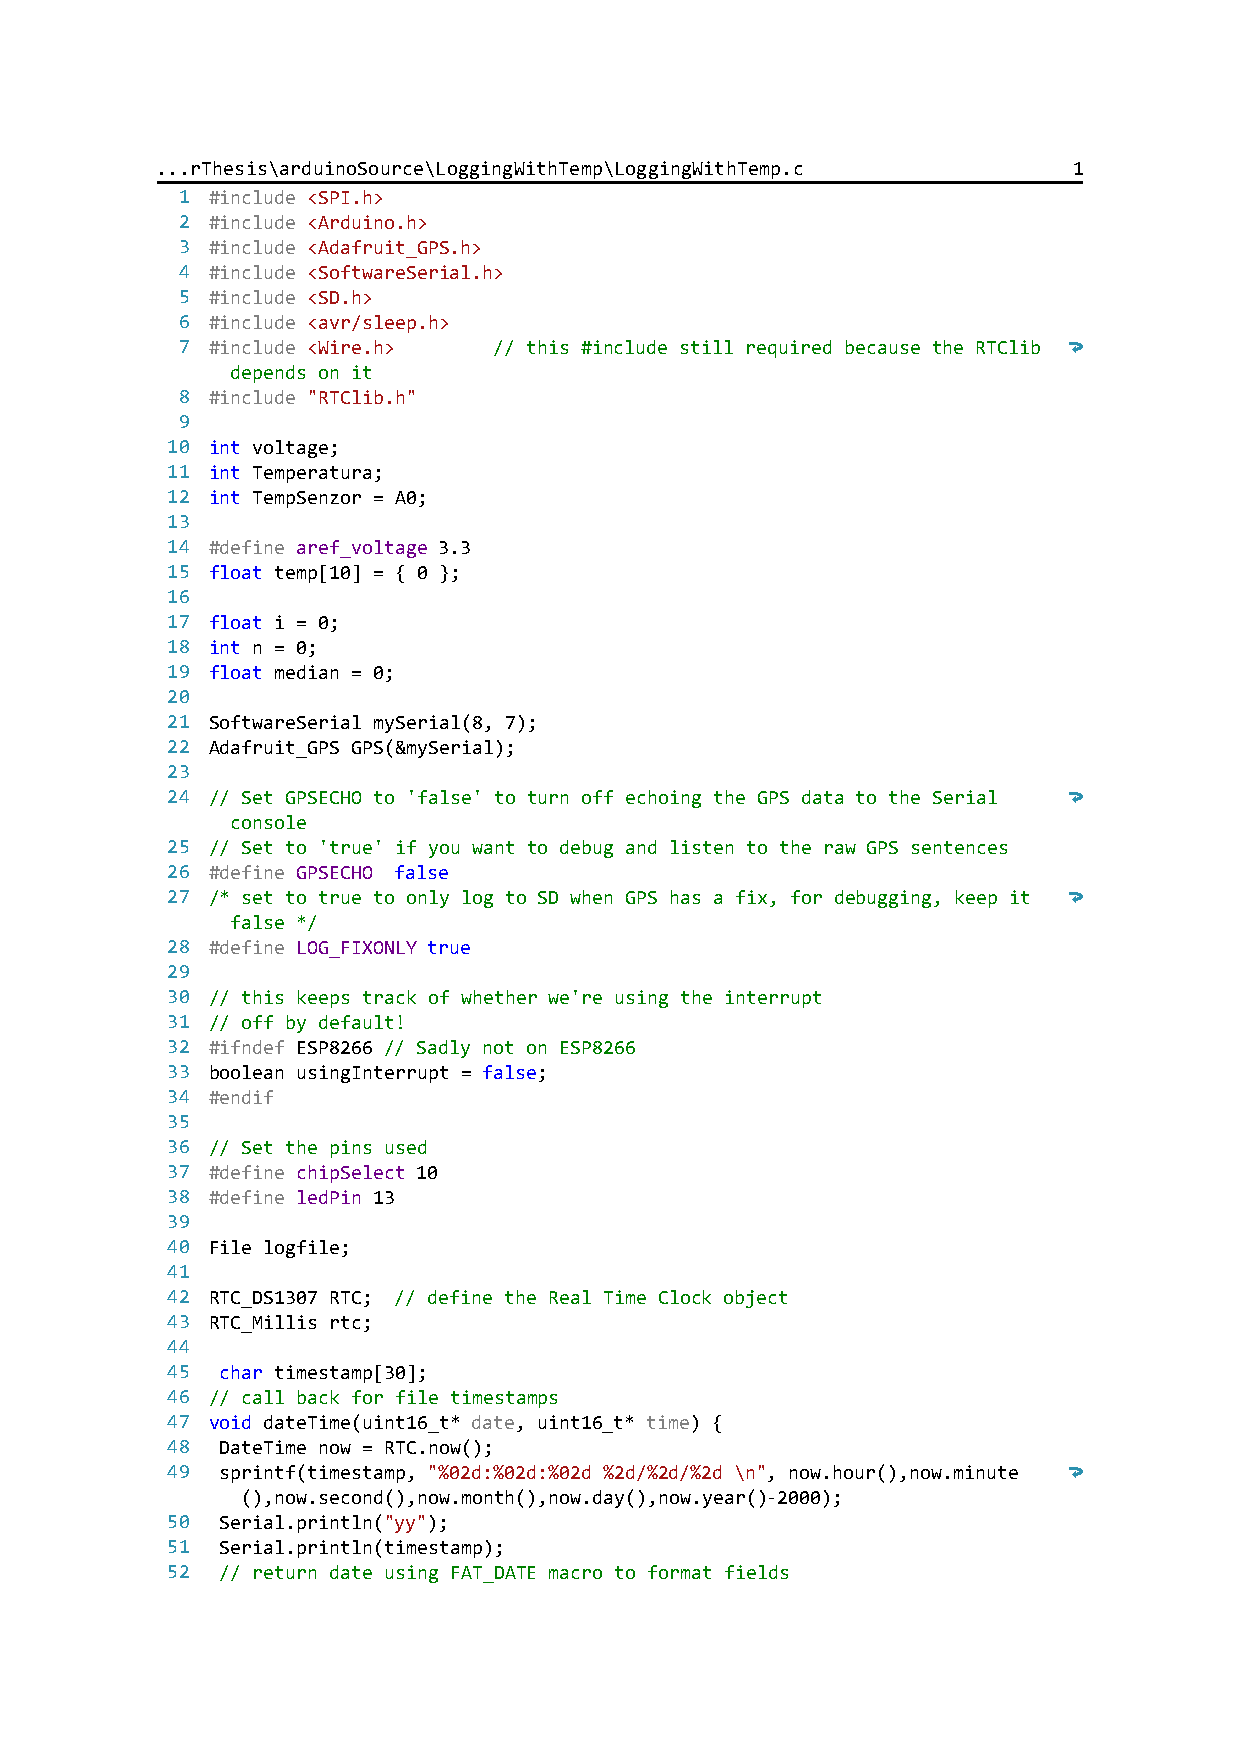
\includepdf[fitpaper, pages=-]{../arduinoSource/LoggingWithTemp/arduinoSource.pdf}
\chapter{Analiza podataka kretanja vozila}\label{AnalizaKretanjaVozila}
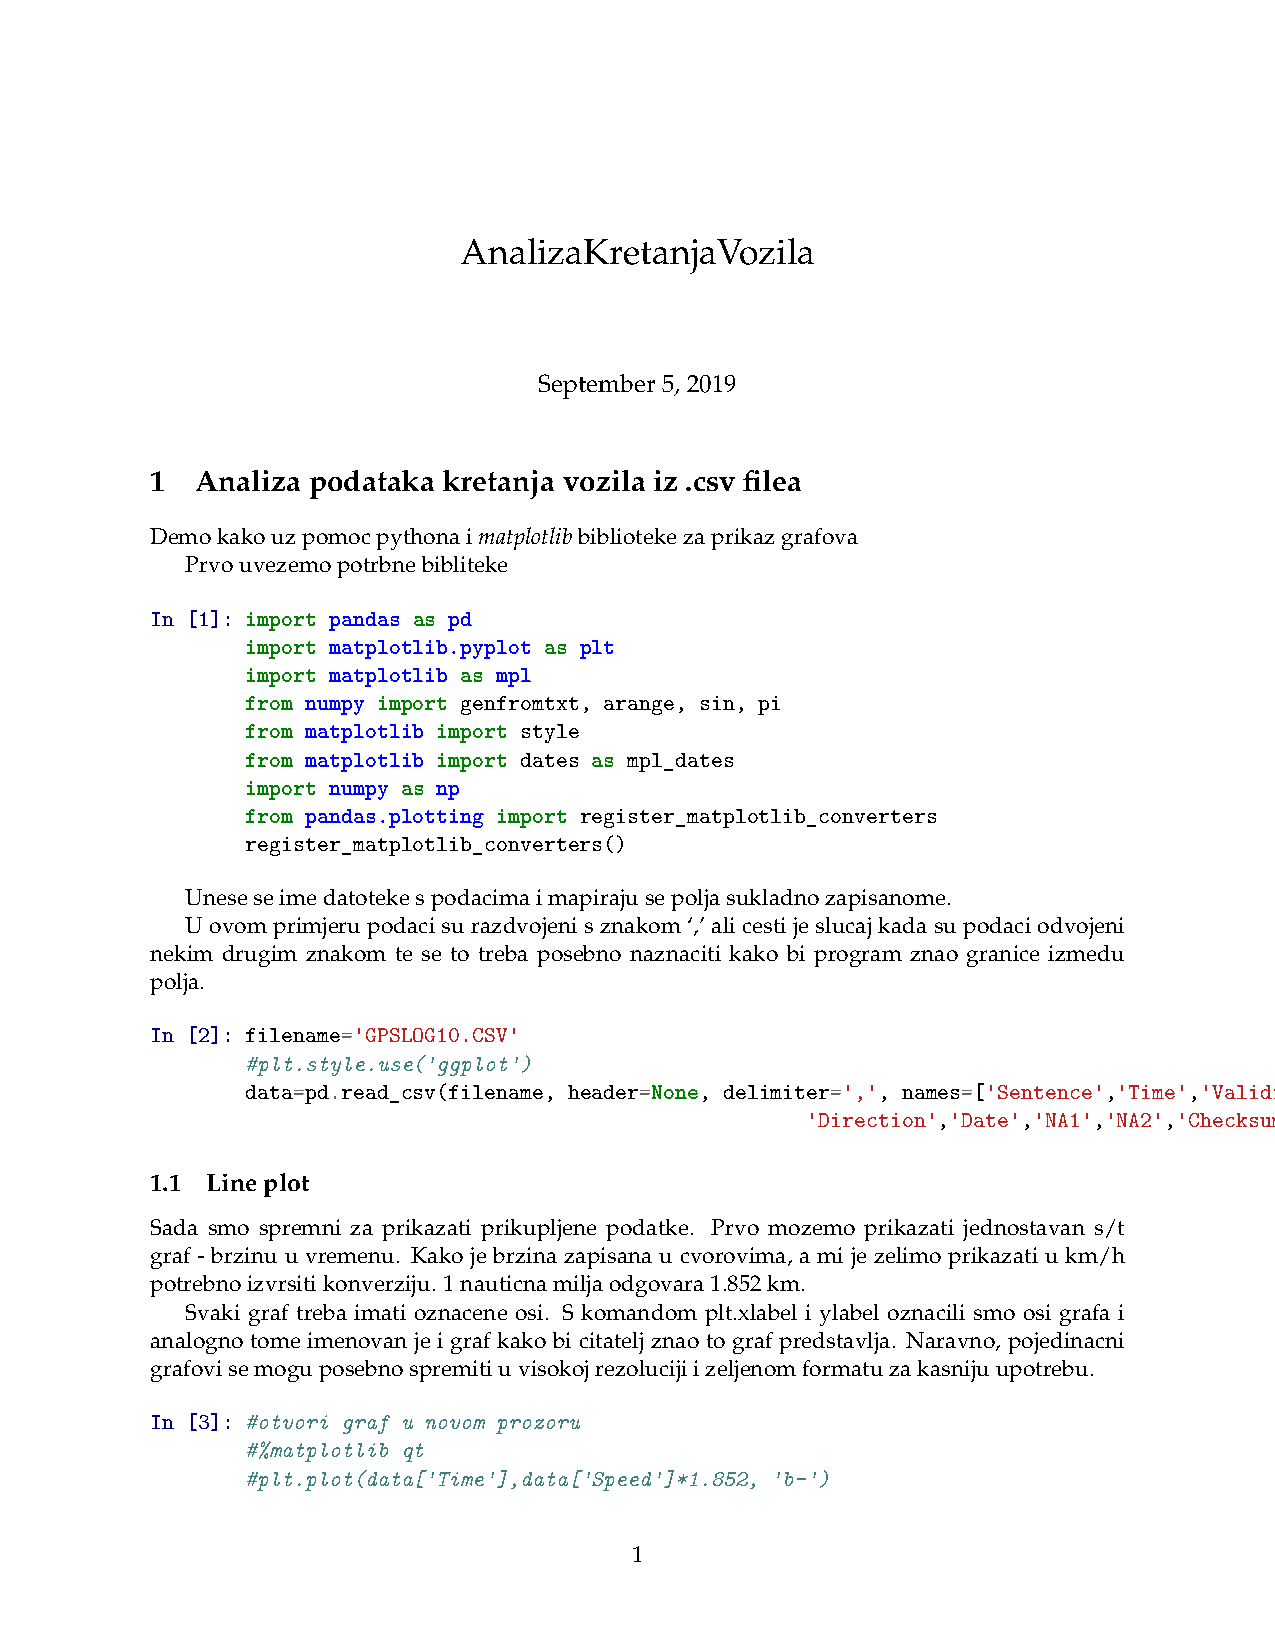
\includepdf[fitpaper, pages=-]{../dataAnalysis/AnalizaKretanjaVozila.pdf}
\chapter{Vizualizacija podataka kretanja lifta}\label{VizualizacijaKretanjaLifta}
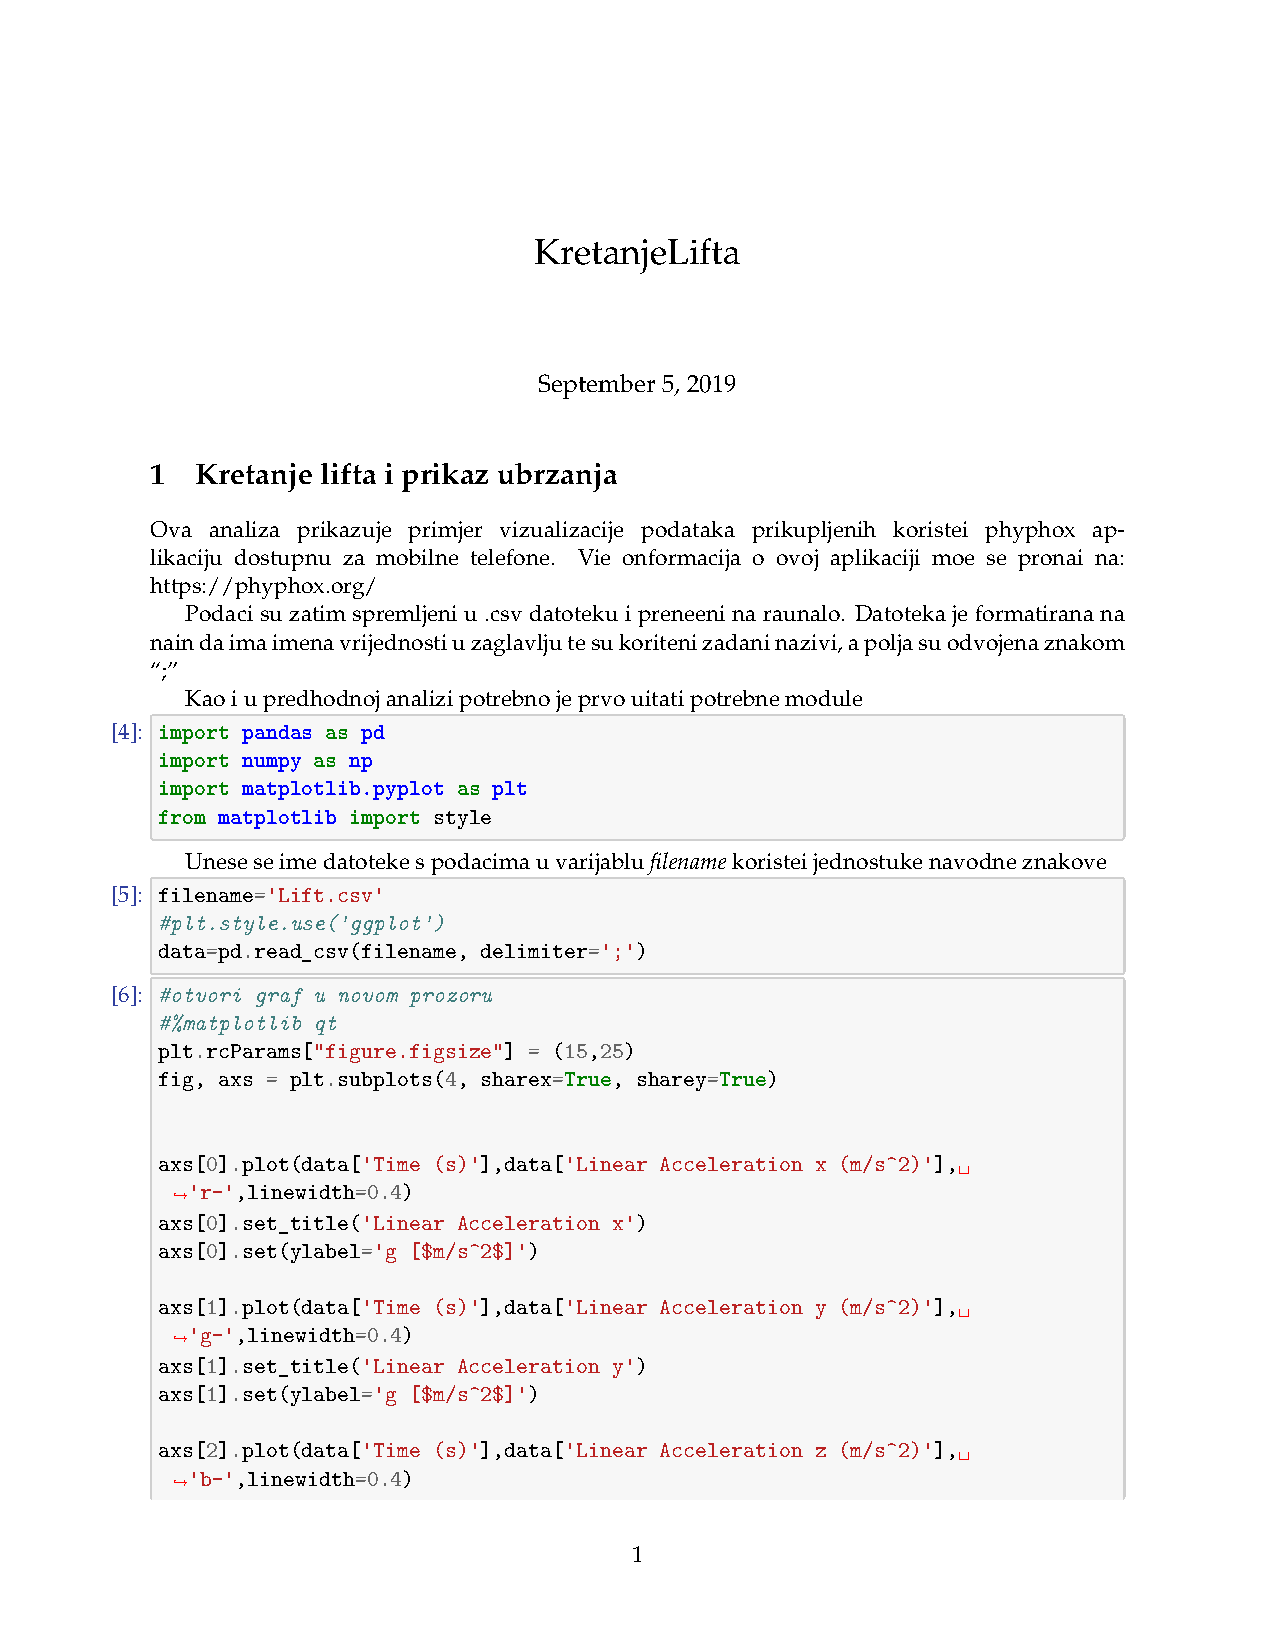
\includepdf[fitpaper, pages=-]{../dataAnalysis/KretanjeLifta.pdf}
\end{appendices}

\end{document}